\section{Riferimenti: lvalues \& rvalues}

Un riferimento, analogamente a un puntatore, archivia l'indirizzo di un oggetto che si trova in un'altra posizione in memoria. A differenza di un puntatore, dopo l'inizializzazione non è possibile impostare un riferimento in modo che indichi un oggetto diverso o che sia impostato su Null. 
Esistono due tipi di riferimenti e operatori:
\begin{itemize}
    \item L'operatore \verb|&| indica: riferimenti \verb|lvalue| che fanno riferimento a una variabile denominata
    \item L'operatore \verb|&&| indica: riferimenti \verb|rvalue|, o un riferimento universale (\verb|rvalue| o \verb|lvalue|) a seconda del contesto,  che fanno riferimento a un oggetto temporaneo.
\end{itemize}

\begin{lstlisting}[language=C++]
#include <iostream>
using namespace std;

int main(){
    Person myFriend;    //struct with char* Name and Short Age
   
    Person& rFriend = myFriend;

    myFriend.Name = "Bill";
    rFriend.Age = 40;

    cout << rFriend.Name << " is " << myFriend.Age << endl; //Bill is 40
}
\end{lstlisting}

\subsection{lvalues: \&}
È possibile considerare un riferimento lvalue come nome alternativo per un oggetto.
Un riferimento deve essere inizializzato e non può essere modificato.


\subsection{Rvalue: \&\&}
I riferimenti Rvalue supportano l'implementazione della semantica di spostamento, che può aumentare significativamente le prestazioni delle applicazioni. La semantica di spostamento, \verb|move()|, consente di scrivere codice per il trasferimento delle risorse (ad esempio memoria allocata in modo dinamico) da un oggetto a un altro.
L’idea è che la proprietà di dati allocati nella memoria dinamica venga trasferita senza dover essere copiata. Lo scopo è aumentare l’efficienza del programma copiando meno dati possibili.

Per implementare la move semantics si fornisce:
\begin{itemize}
    \item costruttore di spostamento
    \item operatore di assegnazione di spostamento \verb|operator=| alla classe
    \item distruttore
\end{itemize}

\begin{lstlisting}[language=C++]
#include <iostream>
using namespace std;

int main(){
    int& x=6; //non compila
    const int& x=6; //compila
    //Dal c++11
    int&& i=7; // rvalue reference, Permette di fare riferimento ad un rvalue e di modificarlo
}
\end{lstlisting}
le reference usuali \verb|int \&| sono lvalue references.

Per comprendere meglio la semantica di spostamento, si consideri l'esempio dell'inserimento di un elemento in un oggetto \verb|vector|. Se viene superata la capacità dell'oggetto, l'oggetto \verb|vector| deve riallocare memoria sufficiente per i relativi elementi e quindi copiare ogni elemento in un'altra posizione di memoria per liberare spazio per l'elemento inserito. Quando un'operazione di inserimento copia un elemento, crea prima di tutto un nuovo elemento. Chiama quindi il costruttore di copia per copiare i dati dall'elemento precedente al nuovo elemento. Infine, elimina definitivamente l'elemento precedente. La semantica di spostamento consente di spostare gli oggetti direttamente senza dover eseguire operazioni di allocazione di memoria e copia costose.


\subsection{Value Categories}

\begin{itemize}
    \item \verb|glvalue|, general lvalue espressione la cui valutazione determina l'identità di un oggetto, di un campo di bit o di una funzione.
    \item \verb|prvalue|, pure rvalue espressione la cui valutazione inizializza un oggetto o un campo di bit oppure calcola il valore dell'operando di un operatore
    \item \verb|xvalue|, eXpiring value glvalue che denota un oggetto o un campo di bit le cui risorse possono essere riutilizzate, in genere perchè vicino a fine vita
    \item \verb|lvalue| è un glvalue che non è un valore xvalue.
    \item \verb|glvalue| è un prvalue o un valore xvalue.
\end{itemize}

\begin{figure}[h]
    \centering
    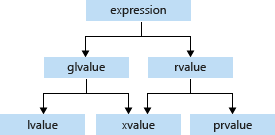
\includegraphics[width=0.4 \textwidth]{img/value.png}
    \caption{Value CategoriesValue}
\end{figure}

Un lvalue ha un indirizzo a cui il programma può accedere, ad esempio nomi di variabili.

Un'espressione prvalue non ha un indirizzo accessibile dal programma. Esempi di espressioni prvalue includono valori letterali, chiamate di funzione che restituiscono un tipo non di riferimento e oggetti temporanei creati durante la valutazione dell'espressione, ma accessibili solo dal compilatore.

Un'espressione xvalue ha un indirizzo che non è più accessibile dal programma, ma può essere usato per inizializzare un riferimento rvalue, che fornisce l'accesso all'espressione. 

\subsection{std::move}
Funzione template che restituisce una rvalue reference al suo argomento. Il suo scopo è "cannibalizzare" l'oggetto per trasferirlo ad un altro riferimento

\begin{lstlisting}[language=c++]
    void swap_copy(T& a, T& b){              void swap_move(T& a, T& b){  
        T& temp(a);                              T& temp(move(a));
        a = b;                                   a = move(b);
        b = temp;                                b = move(temp);
    }                                       }
\end{lstlisting}


\subsection{Default/delete}

È possibile specificare con default and delete
quali di quali metodi adottare la versione di default
e quali non consentire.

\begin{lstlisting}[language=c++]
class A{
    int i;
    public:
    A(const A& _a)=default;
    A(A&& _a):i=0{
        i = _a.i;
        _a.i=0;     //if you want
    }
    A& operator=(const A& _a)=default; //a=(b=c)
    A& operator=(A&& _a){
        i=_a.i;
        _a.i=0;
        return *this;
    }
}; 

\end{lstlisting}